\section{Les factures du cabinet d'infirmières (3 points)}

Une enquête concernant le montant des factures éditées par un important cabinet d'infirmières à permis d'établir l'histogramme suivant :

\begin{center}
	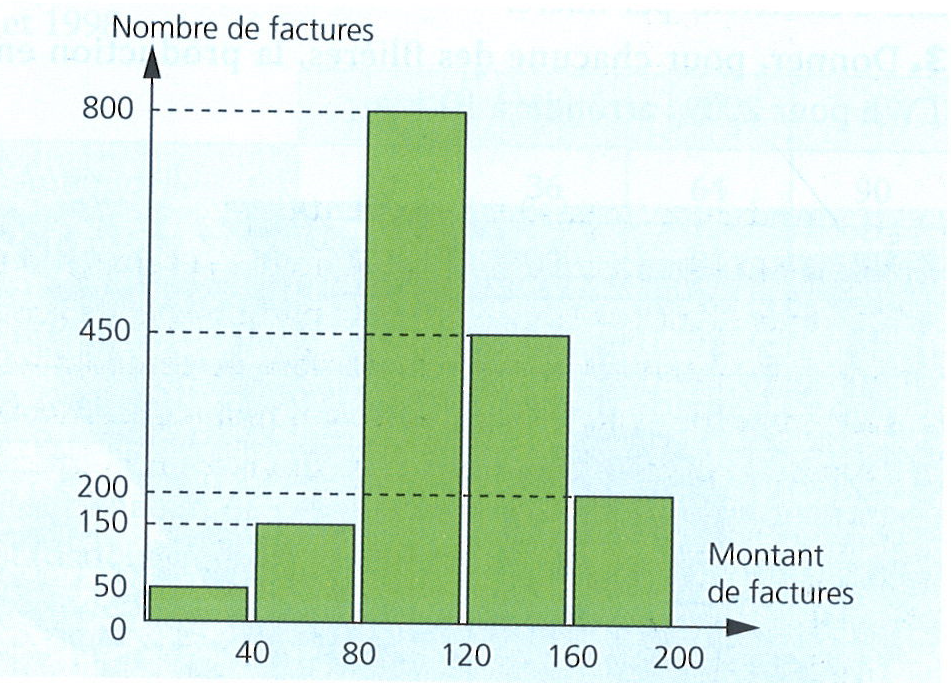
\includegraphics[scale=1]{factures}
\end{center}

Le montant des factures en euro figure en abscisse, l'effectif correspondant $n_i$ figure en ordonnée.

\begin{questions}
	\question[2] Utiliser la figure pour construire un tableau donnant les classes sous forme d'intervalles et les effectifs correspondants.
	\question[1] Déterminer le pourcentage de factures strictement inférieures à 80 €.
\end{questions}